\chapter{Analisi di Algoritmi}
\thispagestyle{chapterInit}
\section{Modelli di calcolo}
    \subsection{Definizioni}    
        \subsubsection{Complessità}
            \begin{definition}
                La \textbf{complessità} di un algoritmo è definita come la quantità di \textbf{tempo} necessaria per eseguirlo in funzione della \textbf{dimensione dell'input}.
            \end{definition}
            Le domande spontanee che ci si pone sono dunque:
            \begin{itemize}
                \item Come definire la dimensione dell'input?
                \item Come misurare il tempo?
            \end{itemize}
        \subsubsection{Dimensione dell'input}
            \begin{definition}
                Per definire la \textbf{dimensione dell'input} abbiamo due criteri:
                \begin{description}
                    \item[Costo Logaritmico] Il costo logaritmico è definito come il numero di bit necessari per rappresentare l'input.
                    \item[Costo Uniforme] La taglia dell'input è definita come il numero di elementi da cui è composto. 
                \end{description}
            \end{definition}
            Ma in molti casi possiamo assumere che tutti gli elementi siano rappresentati dallo stesso numero di bit costante e che coincidono a meno di costante moltiplicativa
        \subsubsection{Tempo}
            \begin{definition} 
                Un'istruzione si considera elementare se può essere eseguita in tempo "costante" dal processore, dunque un esempio ne è la moltiplicazione o una funzione matematica ad esempio $\cos(d)$, ma una istruzione come il massimo tra due numeri non è elementare.
            \end{definition}
        \subsubsection{Modello di calcolo}
            \begin{definition}
                Un modello di calcolo è definito come la rappresentazione astratta di un calcolatore che rispetta i seguenti criteri:
                \begin{description}
                    \item[Astrazione] Il modello deve permettere di nascondere i dettagli.
                    \item[Realismo] Il modello deve riflettere una situazione reale.
                    \item[Potenza Matematica] Il modello deve permettere di dimostrare "formalmente" la complessità di un algoritmo.    
                \end{description}
            \end{definition}
            Esempio di modello di calcolo è la \textbf{Macchina di Turing}.
    \subsection{Esempi di Analisi}
        \subsubsection{Tempo di calcolo $\min()$}
            Sappiamo che ogni istruzione richiede un tempo costante per essere eseguita e che ogni operazione potenzialmente ha una costante diversa dalle altre e che ogni istruzione viene eseguita un numero di volte diversa dalle altre.
            
            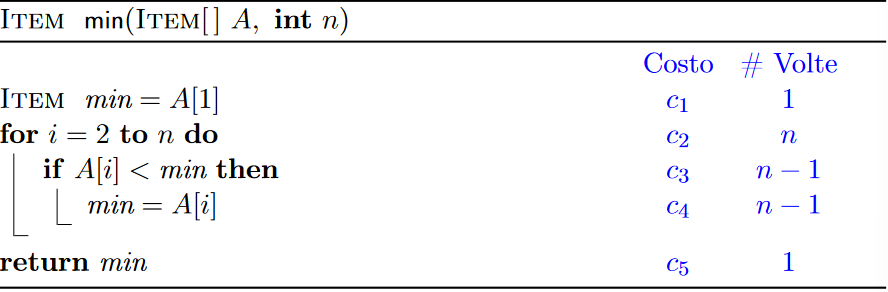
\includegraphics[width=0.9\textwidth]{01/calcoloMin.png}
            
            Otteniamo quindi che il tempo di calcolo è:
            \[
                \begin{aligned}
                    T(n)=&c_1+c_2n+c_3(n-1)+c_4(n-1)+c_5\\
                    =&(c_2+c_3+c_4)n+(c_1+c_5-c_3-c_4) = an+b
                \end{aligned}
            \]
        \subsubsection{Tempo di calcolo di $\operatorname{binarySearch}()$}
            In questo algoritmo il vettore viene suddiviso in due parti:
            $ \text{Parte SX: } \left\lfloor(n-1)/2\right\rfloor $ e $ \text{Parte DX: } \left\lfloor n/2\right\rfloor $.
            
            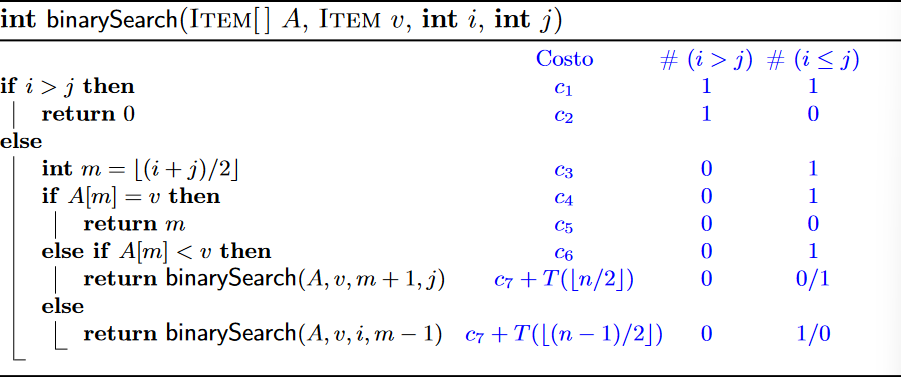
\includegraphics[width=0.9\textwidth]{01/calcoloBinarySearch.png}
            
            A questo punto dobbiamo fare delle assunzioni:
            \begin{itemize}
                \item Assumiamo che la $ n $ potenza di $ 2 $ sia: $ n = 2^k $.
                \item L'elemento cercato non è presente.
                \item Ad ogni passo andiamo sempre a destra in quanto il numero di elementi da valutare è maggiore: $ n/2 $.
            \end{itemize}
            possiamo ora suddividere il problema in due casistiche:
            $$
                \begin{aligned}
                    i>j\quad & (n=0) & T(n)=&c_1 + c_2\\
                    i\leq j\quad & (n>0) & T(n)=&T(n/2) + c_1 + c_2 + c_3 + c_4 + c_6 + c_7\\
                        &&=&T(n/2) + d
                \end{aligned}
            $$
            unendo i due casi otteniamo la \textbf{Relazione di ricorrenza}:
            $$
                T(n)=
                    \begin{cases}
                        c& \text{se } n=0\\
                        T(n/2) +d & \text{se } n>0
                    \end{cases}
            $$
            ottenuta la relazione generalmente per un numero $ n $ di elementi otteniamo che il tempo è dato da:
            $$
                \begin{aligned}
                    T(n)=&T(n/2)+d&\\
                    =&T(n/4)+2d&\\
                    &\hdots\\
                    =&T(1)+kd&\\
                    =&T(0)+(k+1)d&\\
                    =&kd+(c+d) &= d\log n + e
                \end{aligned}
            $$
            ottenendo quindi che il tempo di calcolo è $ O(\log n) $ di natura logaritmica.
    \subsection{Ordini di Complessità}
        \begin{table}[h]
            \centering
            \begin{tabular}{|c|c|c|c|c|c|}
                \hline
                $ f(n) $ & $ n=10^1 $ & $ n=10^2 $ & $n=10^3 $ & $n=10^4 $ & \textbf{Tipo} \\
                \hline
                $ \log n $ & 3 & 6 & 9 & 13 & Logaritmica \\
                \hline
                $ \sqrt{n} $ & 3 & 10 & 31 & 100 & sub-lineare \\
                \hline
                $ n $ & 10 & 100 & 1000 & 10000 & Lineare \\
                \hline
                $ n\log n $ & 30 & 664 & 9965 & 132877 & log-lineare \\
                \hline
                $ n^2 $ & $10^2$ & $10^4$ & $10^6$ & $10^8$ & Quadratica \\
                \hline
                $ n^3 $ & $10^3$ & $10^6$ & $10^9$ & $10^{12}$ & Cubica \\
                \hline
                $ 2^n $ & $1024$ & $10^{30}$ & $10^{301}$ & $10^{3010}$ & Esponenziale\\
                \hline
            \end{tabular}
        \end{table}
\section{Notazione asintotica}
\label{sec:notazioneAsintotica}
    \subsection{Notazioni \texorpdfstring{$ O $, $ \Omega $, $ \Theta $}{O, Omega, Theta}}
        \subsubsection{Notazione $ O $}
            \begin{definition}
                Sia $ g(n) $ una funzione di costo; indichiamo con $ O(g(n)) $ l'insieme delle funzioni $ f(n) $ tali per cui: 
                $$ \exists c>0,\ \exists m\geq 0: f(n) \leq cg(n),\ \forall n\geq m $$
            \end{definition}
            La seguente notazione si legge: $ f(n) $ è "O grande" (big O) di $ g(n) $, con un abuso di notazione si scrive $ f(n)=O(g(n)) $\footnote{\label{fn:note1} Questo è un abuso di notazione in quanto $ O(g(n)) $ è una classe di funzioni e non può essere eguagliata una singola funzione, il simbolo più appropriato sarebbe $ f(n)\in O(g(n)) $}
            . Inoltre per la precedente definizione possiamo dire che $ g(n) $ è un \textbf{limite asintotico superiore} per $ f(n) $, in quanto dopo qualche valore $ m $ la funzione $ g(n) $ è sempre maggiore di $ f(n) $. Inoltre per questo motivo sappiamo che $ f(n) $ cresce al più come $ g(n) $.
        \subsubsection{Notazione $ \Omega $}
            \begin{definition}
                Sia $ g(n) $ una funzione di costo; indichiamo con $ \Omega(g(n)) $ l'insieme delle funzioni $ f(n) $ tali per cui: 
                $$ \exists c>0,\ \exists m\geq 0: f(n) \geq cg(n),\ \forall n\geq m $$
            \end{definition}
            La seguente notazione si legge: $ f(n) $ è "Omega" di $ g(n) $, con un abuso di notazione si scrive $ f(n)=\Omega(g(n)) $\footref{fn:note1}. Inoltre per la precedente definizione possiamo dire che $ g(n) $ è un \textbf{limite asintotico inferiore} per $ f(n) $, in quanto dopo qualche valore $ m $ la funzione $ g(n) $ è sempre minore di $ f(n) $. Inoltre per questo motivo sappiamo che $ f(n) $ cresce almeno come $ g(n) $.
        \subsubsection{Notazione $ \Theta $}
            \begin{definition}
                Sia $ g(n) $ una funzione di costo; indichiamo con $ \Theta(g(n)) $ l'insieme delle funzioni $ f(n) $ tali per cui: 
                $$ \exists c_1>0,\ \exists c_2>0,\ \exists m\geq 0: c_1g(n) \leq f(n) \leq c_2g(n),\ \forall n\geq m $$
            \end{definition}
            La seguente notazione si legge: $ f(n) $ è "Theta" di $ g(n) $, con un abuso di notazione si scrive $ f(n)=\Theta(g(n)) $\footref{fn:note1}. Inoltre per la precedente definizione possiamo dire che $ f(n) $ cresce esattamente come $ g(n) $, detto ciò $ f(n)= \Theta(g(n)) $ se e solo se $ f(n)=O(g(n)) $ e $ f(n)=\Omega(g(n)) $.
        \subsubsection*{Esempio grafico}
            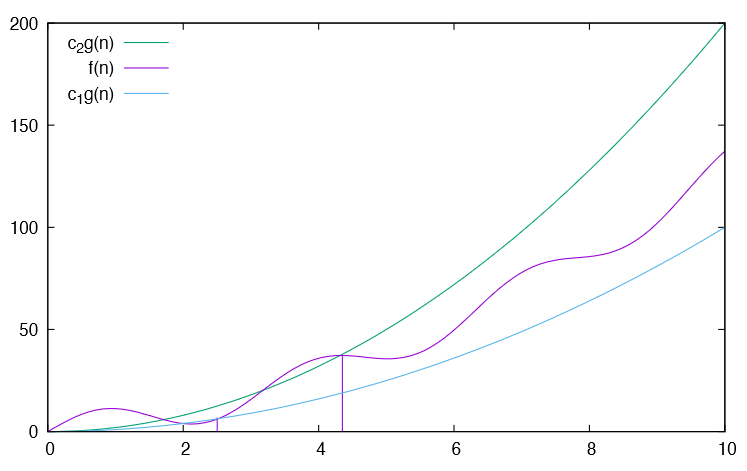
\includegraphics[width=0.5\textwidth]{01/graficoNotazioni.png}
    \subsection{Esempi e Esercizi}
        \subsubsection{Esempio 1}
            $$
                f(n) = 10n^3 + 2n^2 + 7 \stackrel{?}{=} O(n^3)
            $$
            Dobbiamo provare che $ \exists c>0,\ \exists m\geq 0: f(n) \leq cn^3,\ \forall n\geq m $.
            $$
                \begin{aligned}
                    f(n) =& 10n^3 + 2n^2 + 7\\
                    \leq & 10n^3 + 2n^3 + 7 &\quad \forall n \geq 1\\ 
                    \leq & 10n^3 + 2n^3 + n^3 &\quad  \forall n \geq \sqrt[3]{7}\\
                    = & 13 n^3 \stackrel{?}{\leq} cn^3
                \end{aligned}
            $$
            Che è verificata per qualsiasi $ c \geq 13 $ e $ m \geq \sqrt[3]{7} $, arrotondiamo $m$ ad un intero superiore ottenendo $ m = 2 $. 
            
            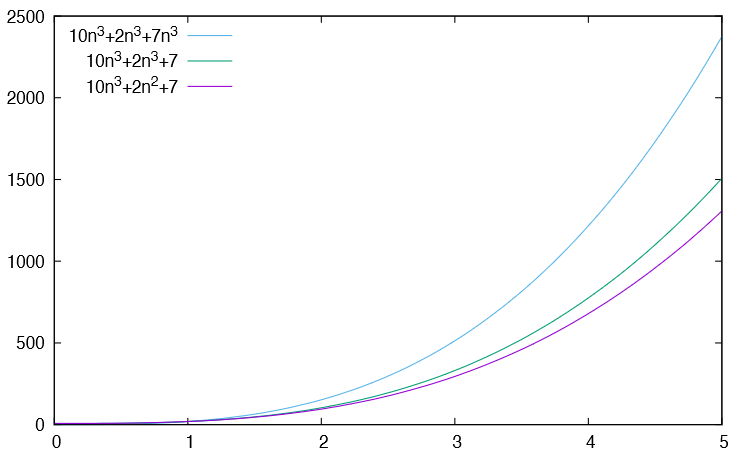
\includegraphics[width=0.5\textwidth]{01/graficoEs1.png}
\section{Complessità problemi v/s algoritmi}
    \subsection{Moltiplicazione numeri complessi}
        Per moltiplicare numeri complessi bisogna svolgere la seguente operazione:
        $$
            (a+bi)(c+di) = [ac-bd]+[ad+bc]i
        $$
        dunque dai parametri $ a,b,c,d $ otteniamo che il risultato da restituire: $ ac-bd $ e $ ad+bc $.
        \paragraph{Domande}
            Considerando che addizioni e sottrazioni costino $ c_1 = 0.01 $ e moltiplicazione costi $ c_2 = 1 $ possiamo chiederci:
            \begin{itemize}
                \item Quanto costa l'algoritmo?
                \item Si può fare meglio?
                \item Qual'è il ruolo del modello di calcolo?
            \end{itemize}
            Dato che si devono fare almeno 4 moltiplicazioni e 2 somme otteniamo che il costo totale è $ 4c_2 + 2c_1 = 4.02 $.
            
            Ora si può fare meglio? La risposta è no in quanto se si potesse fare meglio si potrebbe fare meglio allora bisognerebbe trovare un algoritmo che esegua meno di 4 moltiplicazioni e 2 somme, ma per fare ciò bisognerebbe cambiare il modello di calcolo.
    \subsection{Sommare numeri binari}
        \subsubsection{Algoritmo elementare della somma - $ \operatorname{sum}() $}
            Ipotizziamo che l'operazione da fare sia la somma di due bit singoli e generare il riporto, assegniamo a questa operazione costo $ c $.
            Dopo ciò indichiamo con $ n $ il numero massimo di bit tra i due numeri da sommare, otteniamo dunque che:
            \begin{itemize}
                \item Richiede di esaminare tutti gli $ n $ bit
                \item Costo totale $ cn = O(n) $
            \end{itemize}
        \subsubsection{Esiste allora un algoritmo più efficiente?}
            La risposta è no in quanto se esistesse un algoritmo di tale genere allora potremmo cambiare un solo bit di uno dei due numeri e ottenere un risultato diverso senza che l'algoritmo lo vada ad analizzare, il che è impossibile.
    \subsection{Moltiplicare numeri binari}
        \subsubsection{Algoritmo elementare del prodotto - $\operatorname{prod}()$}
            L'operazione elementare per moltiplicare due numeri binari è la seguente:
            $$
                \begin{array}{c c c c c c c c c c c c c c c}
                    & & & & & & & 1 & 0 & 1 & 1 & 1 & 0 & 1 & *\\
                    & & & & & & & 1 & 1 & 0 & 1 & 1 & 1 & 0 & \\
                    \hline
                    & & & & & & & 0 & 0 & 0 & 0 & 0 & 0 & 0 &\\
                    & & & & & & 1 & 0 & 1 & 1 & 1 & 0 & 1 & &\\
                    & & & & & 1 & 0 & 1 & 1 & 1 & 0 & 1 & & &\\
                    & & & & 1 & 0 & 1 & 1 & 1 & 0 & 1 & & & &\\
                    & & & 0 & 0 & 0 & 0 & 0 & 0 & 0 & & & & &\\
                    & & 1 & 0 & 1 & 1 & 1 & 0 & 1 & & & & & &\\
                    & 1 & 0 & 1 & 1 & 1 & 0 & 1 & & & & & & &\\
                    \hline
                    1 & 0 & 0 & 1 & 1 & 1 & 1 & 1 & 1 & 1 & 0 & 1 & 1 & 0\\
                \end{array}
            $$
            deduciamo che:
            \begin{itemize}
                \item Dobbiamo accedere a tutti i bit
                \item Il costo totale è $ cn^2 = O(n^2) $ perché dobbiamo fare $ n $ somme di $ n $ bit.
            \end{itemize}
        \subsubsection{Soluzione Divide-et-impera}
            La base del principio \textbf{Divide-et-impera} è la seguente:
            \begin{description}
                \item[Divide] Dividere il problema in sotto-problemi più piccoli.
                \item[Impera] risolvi i sotto-problemi in modo ricorsivo.
                \item[Combina] combina le soluzioni dei sotto-problemi per ottenere la soluzione del problema originale.  
            \end{description}
            La soluzione divide-et-impera per il problema della moltiplicazione binaria è la seguente:
            $$
                \begin{aligned}
                    \begin{aligned}
                        X=& a\cdot 2^{n/2} + b\\
                        Y=& c\cdot 2^{n/2} + d\\
                        XY =& ac\cdot 2^n + (ad+bc)\cdot 2^{n/2} + bd
                    \end{aligned}
                    &\quad
                    \begin{aligned}
                        X &= \stackrel{a}{\text{Parte SX}}\quad \stackrel{b}{\text{Parte DX}}\\
                        Y &= \stackrel{c}{\text{Parte SX}}\quad \stackrel{d}{\text{Parte DX}}
                    \end{aligned}
                \end{aligned}
            $$
            Ora possiamo scrivere l'algoritmo:
            \begin{algorithm}
                \caption{boolean[ ] pdi(boolean[ ] X, boolean[ ] Y, int n)}\label{alg:pdi}
                \begin{algorithmic}[1]
                    \If{$n=1$}
                        \State \Return $X[1]\cdot Y[1]$
                    \Else
                        \State spezza $X$ in $a$ e $b$ e $Y$ in $c$ e $d$
                        \State \Return pdi($a,c,n/2$)$\cdot 2^n$ + (pdi($a,d,n/2$) + pdi($b,c,n/2$))$\cdot 2^{n/2}$ + pdi($b,d,n/2$)
                    \EndIf
                \end{algorithmic}
            \end{algorithm}
            La funzione di costo associata all'algoritmo è:
            $$
                T(n)=\begin{cases}
                    c_1 & n=1\\
                    4T(n/2)+c_2\cdot n &  n>1
                \end{cases}
            $$
            \textbf{Nota:} moltiplicare per $2^n$ corrisponde a uno shift a sinistra di $n$ posizioni, svolta in tempo lineare.

            Ora in quanto abbiamo $ 4 $ chiamate ricorsive, assumendo che $c_1$ sia il tempo per moltiplicare due bit e che $ c_2 $ sia il tempo per sommare due numeri binari otteniamo che il tempo di calcolo è $ c_2 \cdot 4^i \cdot \frac{n}{2^i} = T(1) \cdot 4^{\log_2 n} = c_1 \cdot n^{\log_2 4} = c_1 \cdot n^2 $.
            \subparagraph{Ma allora è possibile fare meglio?}
            Long story short: si in quanto è stato provato nel 2021 l'esistenza di un algoritmo di complessità $ O(n\log n) $. 
\section{Algoritmi di Ordinamento}
    \paragraph{Introduzione} L'obbiettivo di questa sezione è valutare la complessità degli algoritmi in base all'input, in alcuni casi gli algoritmi si comportano differentemente in base all'input se siamo a conoscenza dell'input questa ci consente di scegliere un algoritmo più adeguato alla nostra soluzione.
    \paragraph{Come analiziamo gli algoritmi}
        Possiamo analizzare l'efficienza degli algoritmi in base a diversi casi:
        \subparagraph{Caso Pessimo}
            Questa analisi è la più importante in quanto sappiamo che questa restituisce il limite superiore al tempo di esecuzione qualsiasi sia l'input.
        \subparagraph{Caso Medio}
            Questa analisi è la più complessa in quanto bisogna definire il "caso medio" e cosa si intende per "medio", ma è utile con una distribuzione uniforme degli input.
        \subparagraph{Caso Ottimo}
            Utile solo se conosciamo qualcosa sull'input, altrimenti non risulta utile se abbiamo un input arbitrario.
    \subsection{Selection Sort}
        Algoritmo Selection Sort:
        \begin{algorithm}
            \caption{selectionSort(Item[ ] A, \Int n)}\label{alg:selectionSort}
            \begin{algorithmic}[1]
                \For{$i=1$ \To $n-1$}
                    \State \Int $min \gets \operatorname{min}(A,i,n)$
                    \State $A[i]$ $\leftrightarrow$ $\operatorname{min}(A,i,n) $
                \EndFor
            \end{algorithmic}
        \end{algorithm}

        Algoritmo di supporto min:
        \begin{algorithm}
            \caption{int min(Item[ ] A, \Int i, \Int n)}\label{alg:min}
            \begin{algorithmic}[1]
                \State \Int min $\gets i$
                \For{$j=i+1$ \To $n$}
                    \If{$A[j]<A[min]$}
                        \State min $\gets j$
                    \EndIf
                \EndFor
                \State \Return min
            \end{algorithmic}
        \end{algorithm}
        Avendo analizzato il seguente algoritmo notiamo come in ogni caso, ottimo, medio e pessimo, il "ciclo" esterno della funzione $ \operatorname{selectionSort}() $ viene eseguito $ n-1 $ volte, mentre il ciclo interno della funzione $ \operatorname{min}() $ viene eseguito $ n-i $ dove $ i $ è il valore dell'iterazione del ciclo esterno, quindi $ n-1 + n-2 + n-3 + \ldots + 1 = \frac{n(n-1)}{2} $ volte, otteniamo quindi che il tempo di calcolo è $ O(n^2) $ in quanto questo si può approssimare a $ \frac{n^2}{2} $.
        $$  
            \sum_{i=1}^{n-1} n-i = \sum_{i=1}^{n-1} i = \frac{n(n-1)}{2}= O(n^2)
        $$
    \subsection{Insertion Sort}
        L'algoritmo di insertion sort è efficiente per ordinare piccoli insiemi, il concetto dietro a questo si bassa sull'inserimento dell'elemento preso in analisi al posto giusto.
        
        Algoritmo Insertion Sort:
        \begin{algorithm}
            \caption{insertionSort(Item[ ] A, \Int n)}\label{alg:insertionSort}
            \begin{algorithmic}[1]
                \For{$i=2$ \To $n$}
                    \State Item $temp \gets A[i]$
                    \State \Int $j \gets i$
                    \While{$j>1$ and $A[j-1]>temp$}
                        \State $A[j] \gets A[j-1]$
                        \State $j \gets j-1$
                    \EndWhile
                    \State $A[j] \gets temp$
                \EndFor
            \end{algorithmic}
        \end{algorithm}
        
        Il costo di esecuzione non dipende esclusivamente dalla dimensione ma anche dall'ordine degli elementi in ingresso.
        \subparagraph{Caso Pessimo} Il costo dunque nel \textbf{caso pessimo} è $ O(n^2) $ in quanto vengono eseguiti $ n-1 $ cicli esterni e $ n-1 $ cicli interni, ottenendo dunque $ (n-1) + (n-2) + \ldots + 1 = \frac{n(n-1)}{2} = O(n^2) $.
        \subparagraph{Caso Medio }Nel \textbf{caso medio} il costo rimane $ O(n^2) $ in quanto il ciclo interni viene eseguito $ n/2 $ volte, ottenendo dunque $ \frac{n(n-1)}{4} = O(n^2) $.
        \subparagraph{Caso Ottimo} Nel \textbf{caso ottimo} il costo è $ O(n) $ in quanto il ciclo interno non viene mai eseguito.
        
        Questo ci porta a dire che il $ \operatorname{insertionSort}() $ è un algoritmo di ordinamento utile nei casi in cui l'input è già ordinato o quasi ordinato, nei casi nei quali non conosciamo la natura dell'input è meglio utilizzare un algoritmo di ordinamento differente.
    \subsection{Merge Sort}
        L'algoritmo di $ \operatorname{mergeSort}() $ è un algoritmo di ordinamento basato sul principio \textbf{divide-et-impera}.
        \begin{description}
            \item[Divide:] Spezza virtualmente il vettore di $ n $ elementi in sotto-vettori di $ n/2 $ elementi.
            \item[Impera:] Chiama $ \operatorname{mergeSort}() $ ricorsivamente sui due sotto-vettori.
            \item[Combina:] Unisci (\textbf{merge}) i due sotto-vettori ordinati in un unico vettore ordinato. 
        \end{description}
        In input si ha:
        \begin{itemize}
            \item $ A $: vettore di $ n $ elementi.
            \item $ \text{start}, \text{end}, \text{mid} $ sono tali che $ 1\leq \text{start} < \text{mid} < \text{end} \leq n $.
            \item I sotto-vettori $ A[\text{start},\ldots,\text{mid}] $ e $ A[\text{mid}+1,\ldots,\text{end}] $ sono ordinati.
        \end{itemize}
        In output si hanno i due sotto-vettori fusi in un unico sotto-vettore ordinato, tramite un vettore di appoggio $ B $.

        Funzione di appoggio $\operatorname{Merge}$:
        \begin{algorithm}
            \caption{Merge(Item[ ] A, \Int start, \Int end, \Int mid)}\label{alg:merge}
            \begin{algorithmic}[1]
                \State \Int $i,j,k,h$
                \State \Int $i \gets \text{start}$
                \State \Int $j \gets \text{mid}+1$
                \State \Int $k \gets \text{start}$
                \While {$i \leq \text{mid}$ and $j \leq \text{end}$}
                    \If{$A[i] \leq A[j]$}
                        \State $B[k] \gets A[i]$
                        \State $i \gets i+1$
                    \Else
                        \State $B[k] \gets A[j]$
                        \State $j \gets j+1$
                    \EndIf
                    \State $k \gets k+1$
                \EndWhile
                \State $j \gets \text{end}$
                \For {$h=\text{mid}$ \DownTo $i$}
                    \State $A[j] \gets A[h]$
                    \State $j \gets j-1$
                \EndFor
                \For {$j=\text{start}$ \To $k-1$}
                    \State $A[j] \gets B[j]$
                \EndFor
            \end{algorithmic}
        \end{algorithm}
        
        Il costo computazionale di $ \operatorname{Merge}() $ è $ O(n) $, questa è la base del costo computazionale di $ \operatorname{mergeSort}() $.
        \newpage % Usato per evitare che l'algoritmo venga spezzato tra due pagine diverse
        Funzione completa $ \operatorname{mergeSort}() $:

        \begin{algorithm}
            \caption{mergeSort(Item[ ] A, \Int start, \Int end)}\label{alg:mergeSort}
            \begin{algorithmic}[1]
                \If{$\text{start}<\text{end}$}
                    \State \Int $mid \gets (\text{start}+\text{end})/2$
                    \State mergeSort($A,\text{start},\text{mid}$)
                    \State mergeSort($A,\text{mid}+1,\text{end}$)
                    \State merge($A,\text{start},\text{end},\text{mid}$)
                \EndIf
            \end{algorithmic}
        \end{algorithm}

        Assumendo per semplificare che $ n = 2^k $ dove $ k $ è un intero allora l'altezza dell'albero è esattamente $ k = \log n $, in questo modo tutti i sotto-vettori hanno dimensione che è potenza di 2.
        Così facendo il costo computazionale di $ \operatorname{mergeSort}() $ è:
        $$
            T(n)=\begin{cases}
                c & n=1\\
                2T(n/2)+dn & n>1
            \end{cases}
        $$
        dove $ c $ è il costo di un'operazione elementare, $ d $ è il costo di $ \operatorname{Merge}() $ e $ n $ è il costo di copiare i valori da $ B $ a $ A $.